% ----- Consignes exo 1
\begin{td-exo}[Distance discrète]\, % 1
    Soit \(X\) un ensemble et \(\delta\) la distance discrète sur cet ensemble. 
    \begin{enumerate}
        \item Vérifier que \(\delta\) est bien une distance sur \(X\).
        \item Déterminer les boules ouvertes et fermées de \((X, \delta)\).
        Puis, déterminer la topologie \(T_\delta\) associée à \(\delta\).
    \end{enumerate}
\end{td-exo}
% ----- Solutions exo 1
\iftoggle{showsolutions}{
    \begin{td-sol}[]\, % 1
        Commençons par rappeler la définition de la distance discrète:
        \begin{equation*}
            \delta(x, y) = \begin{cases}
                0 & \text{si } x = y, \\
                1 & \text{si } x \neq y.
            \end{cases}
        \end{equation*}
        \begin{enumerate}
            \item Vérifions les quatres propriétés d'une distance:
            \begin{enumerate}[label=(\roman*)]
                \item Positivité: \(\forall x, y \in X, \delta(x, y) \geq 0\), vrai par définition.
                \item Séparation: \(\forall x, y \in X, \delta(x, y) = 0 \iff x = y\), vrai par définition.
                \item Symétrie: \(\forall x, y \in X, \delta(x, y) = \delta(y, x)\), vrai par définition.
                \item Inégalité triangulaire: \(\forall x, y, z \in X, \delta(x, y) \leq \delta(x, z) + \delta(z, y)\).
                Si \(x = y\), alors \(\delta(x, y) = 0\) et l'inégalité est vérifiée. Sinon, \(z\neq x\) 
                et \(z\neq y\), donc \(\delta(x, z) = \delta(z, y) = 1\). L'inégalité est donc vérifiée.
            \end{enumerate}

            \item Rappelons que la boule ouverte de centre \(x\in X\) et de rayon \(r > 0\) pour une distance \(d\) est
            \begin{equation*}
                \bolo{x}{r} = \{y \in X \mid d(x, y) < r\}.
            \end{equation*}
            Ici on a plusieurs cas qui se présentent:
            \begin{itemize}
                \item Si \(r \leq 1\), alors \(\bolo{x}{r} = \{y \in X \mid \delta(x,y) < r\} = \{x\}\).
                \item Si \(r > 1\), alors \(\bolo{x}{r} = \{y \in X \mid \delta(x,y) < r\} = X\).
            \end{itemize}

            Pour les boules fermées on a
            \begin{equation*}
                \bolf{x}{r} = \{y \in X \mid d(x, y) \leq r\}.
            \end{equation*}
            Plusieurs cas qui se présentent:
            \begin{itemize}
                \item Si \(r < 1\), alors \(\bolo{x}{r} = \{y \in X \mid \delta(x,y) \leq r\} = \{x\}\).
                \item Si \(r \geq 1\), alors \(\bolo{x}{r} = \{y \in X \mid \delta(x,y) \leq r\} = X\).
            \end{itemize}
        \end{enumerate}
    \end{td-sol}
}{}

% ----- Consignes exo 2
\begin{td-exo}[Distance et normes]\, % 2
    Soit \(E\) un \(\bb K\)-espace vectoriel (avec \(\bb K = \bb Q,\bb R,\bb C\)) et \(\nn{\cdot}\) une norme sur \(E\).
    Montrer que la fonction
    \begin{equation*}
        \begin{aligned}
            d\ \colon\ E \times E &\to \R \\
            (x, y) &\mapsto \nn{y - x}
        \end{aligned}
    \end{equation*}
    définit une distance sur \(E\).
\end{td-exo}
% ----- Solutions exo 2
\iftoggle{showsolutions}{
    \begin{td-sol}[]\, % 2
        Vérifions les quatres propriétés d'une distance:
        \begin{enumerate}[label=(\roman*)]
            \item Positivité: \(\forall x, y \in E, d(x, y) = \nn{y - x} \geq 0\) car la norme est positive.
            \item Séparation: \(\forall x, y \in E, d(x, y) = 0 \iff \nn{y - x} = 0 \iff y - x = 0 \iff y = x\).
            \item Symétrie: \(\forall x, y \in E, d(x, y) = \nn{y - x} = \nn{x - y} = d(y, x)\).
            \item Inégalité triangulaire: \(\forall x, y, z \in E, d(x, y) = \nn{y - x} \leq \nn{y - z} + \nn{z - x} = d(x, z) + d(z, y)\)
            par l'inégalité triangulaire de la norme.
        \end{enumerate}
    \end{td-sol}
}{}

% ----- Consignes exo 3
\begin{td-exo}[Normes sur \(\R^n\)]\, % 3
    Soit \(x = (x_1,\ldots,x_n)\) un vecteur de \(\R^n\). Montrer que les fonctions suivantes définissent des normes sur \(\R^n\):
    \begin{equation*}
        \begin{aligned}
            N_1\ \colon\ \R^n &\to \R \\
            x &\mapsto \sum_{i=1}^n \abs{x_i},
        \end{aligned}
        \qquad\text{et}\qquad
        \begin{aligned}
            N_\infty\ \colon\ \R^n &\to \R \\
            x &\mapsto \max_{1 \leq i \leq n} \left(\abs{x_i}\right).
        \end{aligned}
    \end{equation*}
    Dessiner leurs boules unités dans le cas \(n = 2\).
\end{td-exo}
% ----- Solutions exo 3
\iftoggle{showsolutions}{
    \begin{td-sol}[]\, % 3
        Rappelons les propriétés d'une norme:
        \begin{enumerate}[label=(\roman*)]
            \item Positivité: \(\forall x \in \R^n, N(x) \geq 0\), vrai car la somme des valeurs absolues est positive.
            \item Séparation: \(\forall x \in \R^n, N(x) = 0 \iff \sum_{i=1}^n \abs{x_i} = 0 \iff x_i = 0\ \forall i\).
            \item Homogénéité: \(\forall x \in \R^n, \forall \lambda \in \R, N(\lambda x) = \abs{\lambda} \sum_{i=1}^n \abs{x_i} = \abs{\lambda} N(x)\).
            \item Inégalité triangulaire: \(\forall x, y \in \R^n, N(x + y) = \sum_{i=1}^n \abs{x_i + y_i} \leq \sum_{i=1}^n \abs{x_i} + \abs{y_i} = N(x) + N(y)\).
        \end{enumerate}
        Vérifions maintenant que \(N_1\) est une norme:
        \begin{enumerate}[label=(\roman*)]
            \item Positivité: \(\forall x \in \R^n, N_1(x) = \sum_{i=1}^n \abs{x_i} \geq 0\).
            \item Séparation: \(\forall x \in \R^n, N_1(x) = 0 \iff \sum_{i=1}^n \abs{x_i} = 0 \iff x_i = 0\ \forall i\).
            \item Homogénéité: \(\forall x \in \R^n, \forall \lambda \in \R, N_1(\lambda x) = \sum_{i=1}^n \abs{\lambda x_i} = \abs{\lambda} \sum_{i=1}^n \abs{x_i} = \abs{\lambda} N_1(x)\).
            \item Inégalité triangulaire: \(\forall x, y \in \R^n, N_1(x + y) = \sum_{i=1}^n \abs{x_i + y_i} \leq \sum_{i=1}^n \abs{x_i} + \abs{y_i} = N_1(x) + N_1(y)\).
        \end{enumerate}
        Vérifions maintenant que \(N_\infty\) est une norme:
        \begin{enumerate}[label=(\roman*)]
            \item Positivité: \(\forall x \in \R^n, N_\infty(x) = \max_{1 \leq i \leq n} \left(\abs{x_i}\right) \geq 0\).
            \item Séparation: \(\forall x \in \R^n, N_\infty(x) = 0 \iff \max_{1 \leq i \leq n} \left(\abs{x_i}\right) = 0 \iff x_i = 0\ \forall i\).
            \item Homogénéité: \(\forall x \in \R^n, \forall \lambda \in \R, N_\infty(\lambda x) = \max_{1 \leq i \leq n} \left(\abs{\lambda x_i}\right) = \abs{\lambda} \max_{1 \leq i \leq n} \left(\abs{x_i}\right) = \abs{\lambda} N_\infty(x)\).
            \item Inégalité triangulaire: \(\forall x, y \in \R^n, N_\infty(x + y) = \max_{1 \leq i \leq n} \left(\abs{x_i + y_i}\right) \leq \max_{1 \leq i \leq n} \left(\abs{x_i}\right) + \max_{1 \leq i \leq n} \left(\abs{y_i}\right) = N_\infty(x) + N_\infty(y)\).
        \end{enumerate}

        Voici leurs boules unités dans le cas \(n = 2\):
        \begin{center}
    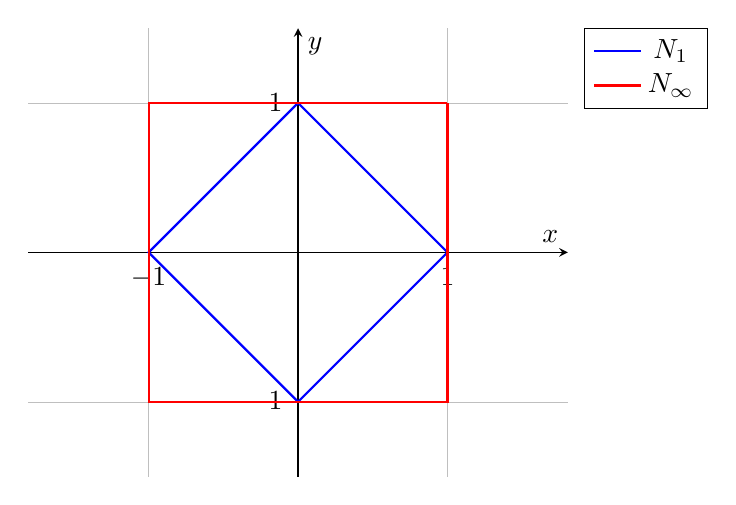
\begin{tikzpicture}
    \begin{axis}[
    axis equal,
    axis lines = middle,
    xmin = -1.5, xmax = 1.5,
    ymin = -1.5, ymax = 1.5,
    xlabel = {$x$},
    ylabel = {$y$},
    xtick = {-1, 0, 1},
    ytick = {-1, 0, 1},
    grid = both,
    major grid style = {line width=.2pt,draw=gray!50},
    minor grid style = {line width=.1pt,draw=gray!20},
    legend pos = outer north east,
    ]
    % Norme 1 (losange)
    \addplot[
    color=blue,
    mark=none,
    thick,
    ] coordinates {
    (1, 0) (0, 1) (-1, 0) (0, -1) (1, 0)
    };
    \addlegendentry{$N_1$}

    % Norme infinie (carré)
    \addplot[
    color=red,
    mark=none,
    thick,
    ] coordinates {
    (1, 1) (-1, 1) (-1, -1) (1, -1) (1, 1)
    };
    \addlegendentry{$N_\infty$}
    \end{axis}
    \end{tikzpicture}
\end{center}


    \end{td-sol}
}{}



% ----- Consignes exo 4
\begin{td-exo}[Distance Fly Emirates]\, % 4
    Soit \((X,d)\) un espace métrique et \(\omega\) un point fixé
    de \(X\) (Dubaï). On définit la fonction suivante:
    \begin{equation*}
        \begin{aligned}
            D\ \colon\ X \times X &\to \R \\
            (x, y) &\mapsto \begin{cases}
                0 & \text{si } x = y, \\
                d(x, \omega) + d(\omega, y) & \text{si } x \neq y.
            \end{cases}
        \end{aligned}
    \end{equation*}
    \begin{enumerate}
        \item Montrer que \(D\) définit une distance sur \(X\).
        \item On suppose que \((X,d) = (\R^2, d_2)\) et \(\omega = (0,0)\).
        Pour \(a\in X\), dessiner les boules ouvertes centrées en \(a\) pour la distance \(D\).
        \item Montrer que si \(x\neq \omega\), le singleton \(\{x\}\) est ouvert pour la distance \(D\).
    \end{enumerate}
\end{td-exo}
% ----- Solutions exo 4
\iftoggle{showsolutions}{
    \begin{td-sol}[]\, % 4
        test
    \end{td-sol}
}{}




